\documentclass[conference]{IEEEtran}
\usepackage{graphicx}
\usepackage{booktabs}
\usepackage{amsmath}
\usepackage{url}
\usepackage{hyperref}

\title{Green Shields, Live Failures: Trust Integrity for LLM Affect Probes}

\author{
\IEEEauthorblockN{Siddarth Boggarapu}
\IEEEauthorblockA{Independent Researcher\\
Bengaluru, India\\
siddarthb078@gmail.com}
}

\begin{document}
\maketitle

\begin{abstract}
Trust interfaces for language-model tools often display green ``safe'' badges after fixture checks.
We study whether such badges remain honest on live claim-encode rows from HaluEval and TruthfulQA.
We introduce Anima, probes for valence, arousal, and uncertainty on Hugging Face causal LMs, plus a
Trust Integrity Gate that seals \texttt{trust\_ui\_claim\_allowed}.
On Qwen2.5-0.5B-Instruct and TinyLlama-1.1B-Chat, Protocol~F AUROC is 1.00 while baseline Protocol~L
collapses (e.g., Qwen--HaluEval AUROC 0.25, never-abstain, anti-aligned ranking); GreenShieldBench denies unlock.
Named Protocol~L$'$ LOQO ridge recovery restores primary-suite AUROC (Qwen--HaluEval 0.92) and unlocks adapted
receipts without silent production label flips.
Matched semantic entropy does not overturn baseline failure.
A Narratives depth check shows encoding ceilings (word-rate max $r$ up to $\sim$0.67) with near-zero PCA$\to$VA
holdout---encoding interest without emotion--brain claims.
\end{abstract}

\begin{IEEEkeywords}
Claim encoding, hallucination evaluation, interpretability, trust user interfaces, valence-arousal probing.
\end{IEEEkeywords}

\section{Introduction}
Product demos wrap LMs in trust UI. Fixture suites can make badges look perfect while live public rows invert ranking,
flatten AUROC, or never abstain.
We treat trust-UI integrity as an evaluation object and release Anima with sealed receipts that refuse green language
without a live unlock.
Contributions: (i)~probe instrumentation; (ii)~Protocols F/L/R/L$'$; (iii)~Trust Integrity Gate and GreenShieldBench;
(iv)~locked negative and named-recovery results; (v)~encoding-only Narratives depth.
We do not claim hallucination SOTA, model feelings, voxel TRIBE, or a human badge study.

\section{Methods}
\subsection{Protocols}
Protocol~F is fixture smoke.
Protocol~L is live claim-encode ($n{=}80$, bootstrap $B{=}2000$, seed 42).
Protocol~L$'$ is leave-one-question-out ridge adaptation---a named operating point, not a silent polarity flip.
\subsection{Trust Integrity Gate}
TIG aggregates AUROC floors, transfer gap $\Delta$(F$-$L), never-abstain, and polarity into
\texttt{trust\_ui\_claim\_allowed}.
Fixture AUROC alone cannot unlock.

\section{Results}
Fig.~\ref{fig:fvl} shows fixture vs live collapse.
Fig.~\ref{fig:lp} shows L$'$ recovery.
Fig.~\ref{fig:badge} shows the sealed claim bit.
Fig.~\ref{fig:fmri} and Fig.~\ref{fig:se} report Narratives ceilings and matched semantic entropy.
Numbers match \texttt{benchmarks/reports/ANIMA\_NUMBER\_TABLE.md}.

\begin{figure}[!t]
\centering
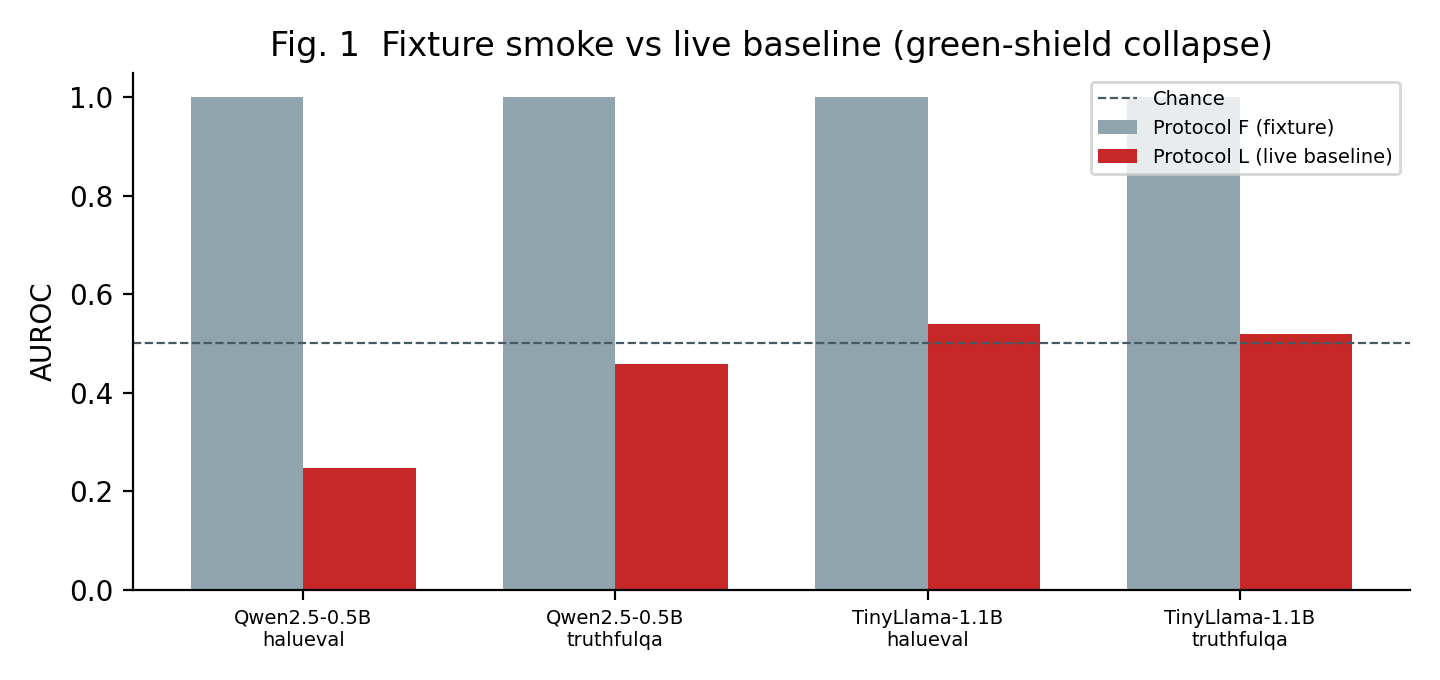
\includegraphics[width=\columnwidth]{figures/fig1_fixture_vs_live.png}
\caption{Protocol F vs Protocol L AUROC (locked rows).}
\label{fig:fvl}
\end{figure}

\begin{figure}[!t]
\centering
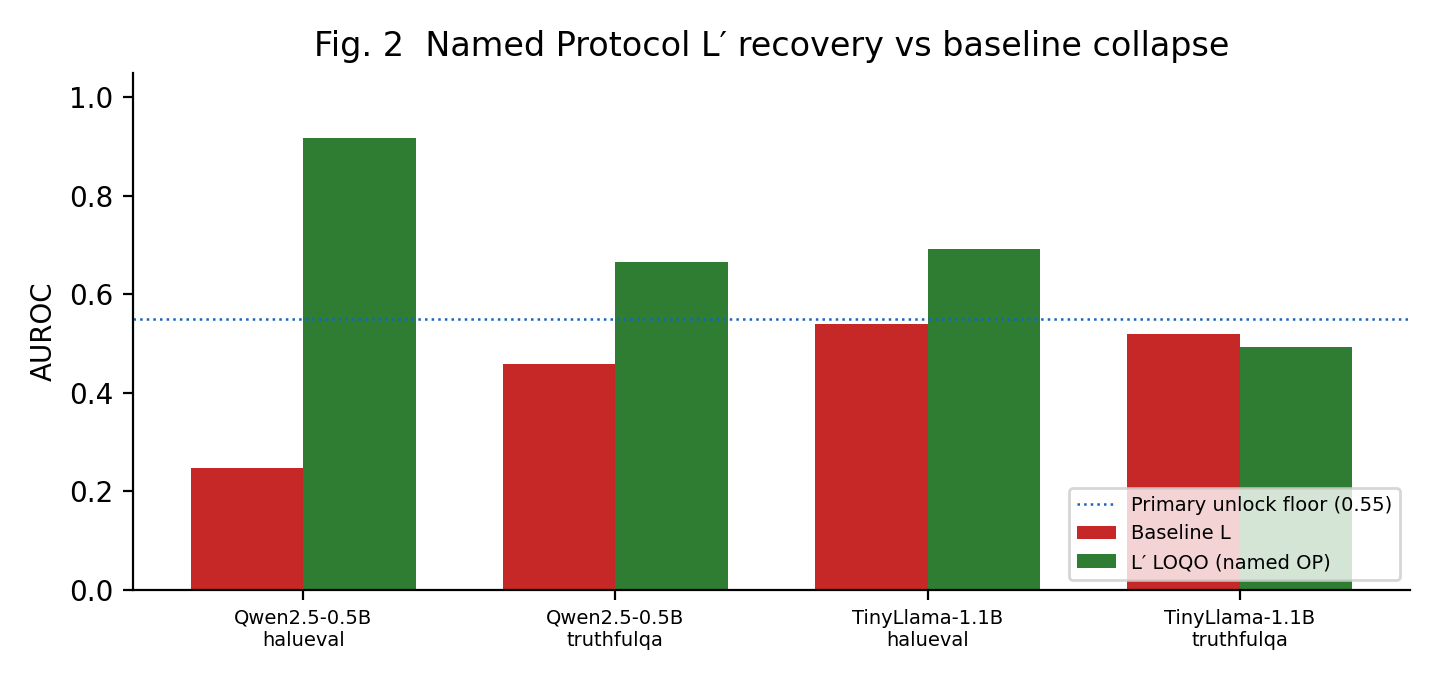
\includegraphics[width=\columnwidth]{figures/fig2_lprime_unlock.png}
\caption{Baseline L vs Protocol L$'$ LOQO AUROC.}
\label{fig:lp}
\end{figure}

\begin{figure}[!t]
\centering
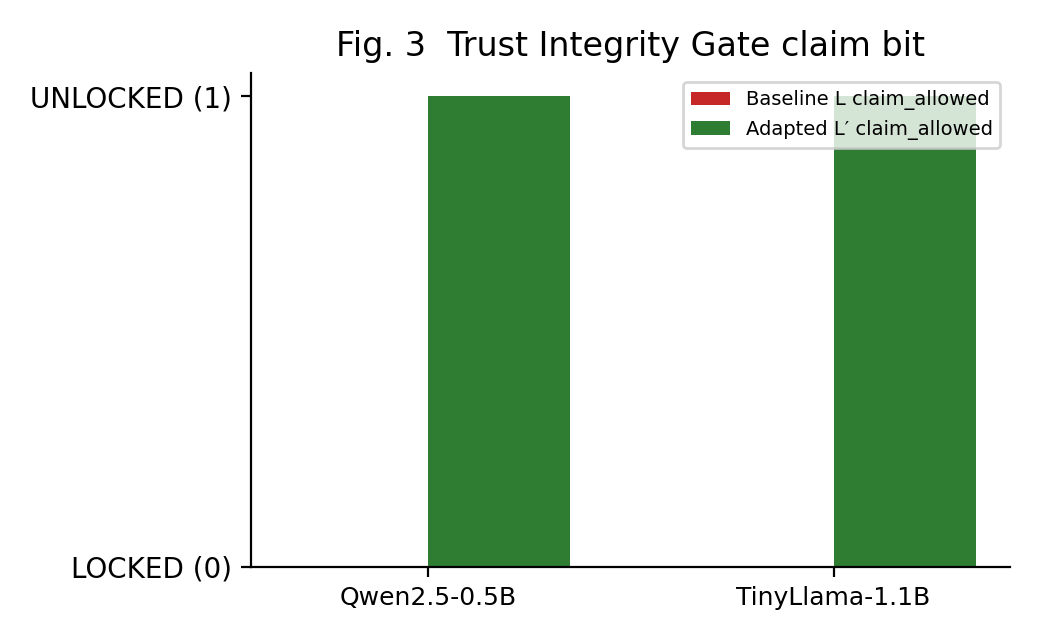
\includegraphics[width=0.9\columnwidth]{figures/fig3_trust_badge.png}
\caption{Trust Integrity Gate claim bit.}
\label{fig:badge}
\end{figure}

\begin{figure}[!t]
\centering
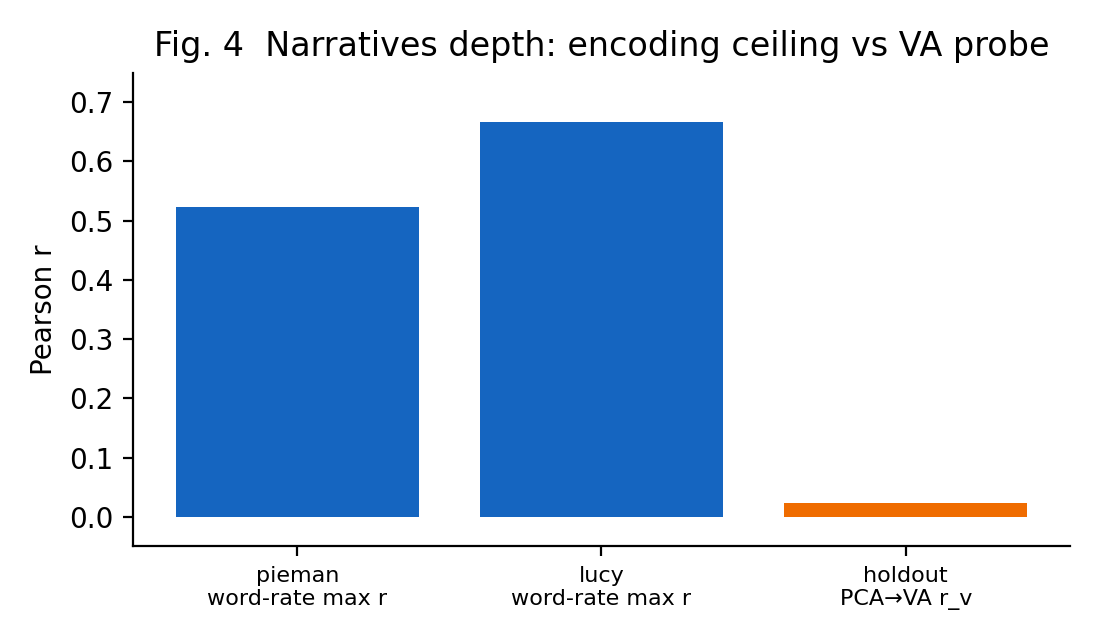
\includegraphics[width=0.9\columnwidth]{figures/fig4_fmri_ceilings.png}
\caption{Narratives encoding ceilings vs PCA$\to$VA holdout.}
\label{fig:fmri}
\end{figure}

\begin{figure}[!t]
\centering
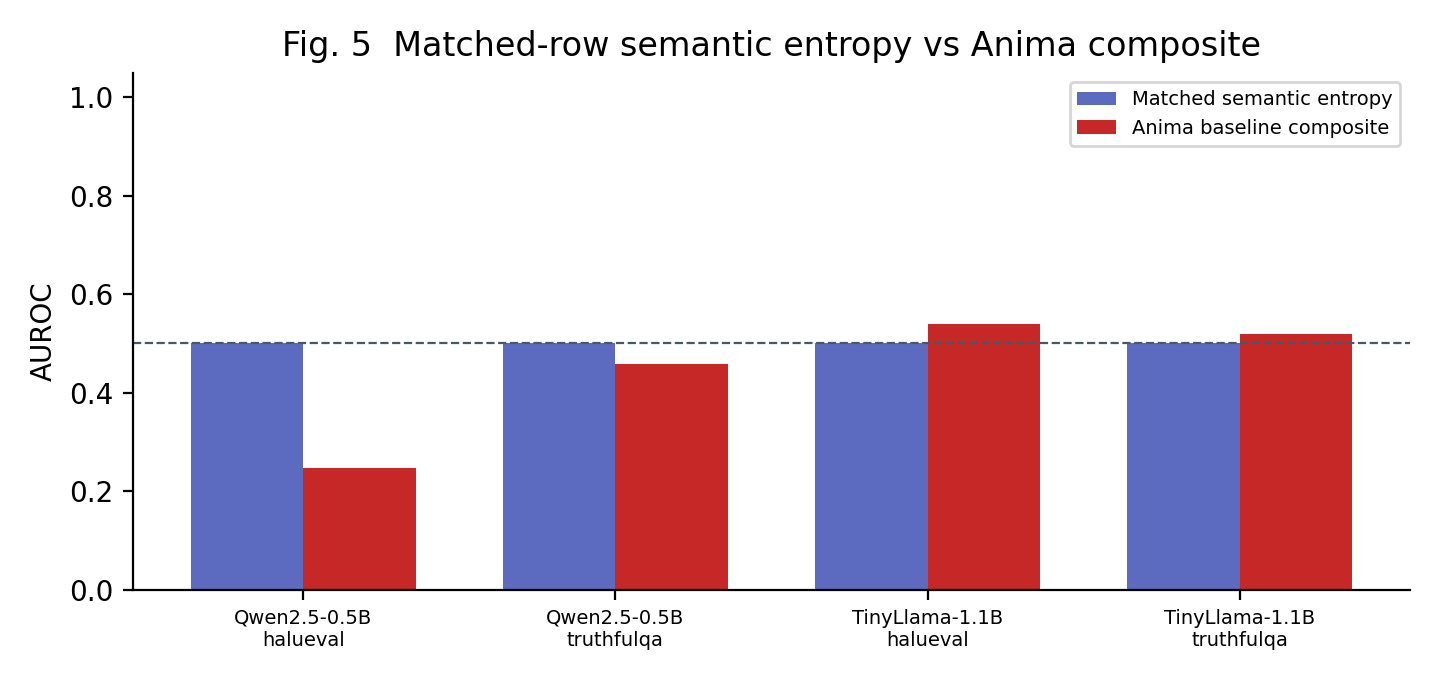
\includegraphics[width=\columnwidth]{figures/fig5_se_matched.png}
\caption{Matched semantic entropy vs Anima composite.}
\label{fig:se}
\end{figure}

\begin{table}[!t]
\caption{Baseline Protocol L AUROC}
\label{tab:l}
\centering
\begin{tabular}{llcc}
\toprule
Model & Suite & AUROC & Polarity \\
\midrule
Qwen & HaluEval & 0.2469 & anti\_aligned \\
Qwen & TruthfulQA & 0.4587 & near\_chance \\
TinyLlama & HaluEval & 0.5387 & near\_chance \\
TinyLlama & TruthfulQA & 0.5188 & near\_chance \\
\bottomrule
\end{tabular}
\end{table}

\section{Limitations}
Claim-encode $\neq$ free-gen+judge.
Misleading-green is simulated.
L$'$ is adaptation.
fMRI subset is two stories $\times$ three subjects.
Scale is two small models by design for lockable honesty.

\section{Conclusion}
Fixture-perfect green shields can fail live.
Anima seals the failure, surfaces it in product UI, and documents named L$'$ recovery without overclaim.

\begin{thebibliography}{00}
\bibitem{kuhn2023} A. Kuhn, Y. Gal, and S. Farquhar, ``Semantic Uncertainty,'' ICLR, 2023.
\bibitem{reforms2024} S. Kapoor et al., ``REFORMS,'' Sci.\ Adv., 2024.
\bibitem{narratives} S.~A. Nastase et al., ``Narratives,'' OpenNeuro ds002345.
\bibitem{halueval} J. Li et al., ``HaluEval,'' EMNLP, 2023.
\bibitem{truthfulqa} S. Lin, J. Hilton, and O. Evans, ``TruthfulQA,'' ACL, 2022.
\end{thebibliography}

\end{document}
